\documentclass[11pt]{article}

\usepackage[spanish,activeacute]{babel}
\usepackage{amsfonts}
\usepackage{graphicx}
\usepackage{whilecode2}


    \title{\textbf{Practica 3}}
    \author{Carmen Alonso Jimenez}
    \date{\today}
    
    \addtolength{\topmargin}{-4cm}
    \addtolength{\textheight}{4cm}
    %\usepackage[spanish]{babel}
    \usepackage[a4paper, margin=3cm, top=5mm, bottom=15mm]{geometry}
    \usepackage{graphicx}
    \usepackage{tikz}

\begin{document}

\maketitle
\thispagestyle{plain}
\setlength{\parskip}{6pt}

\section{Define the TM solution of exercise 3.4 of the problem list and test its correct
behaviour}

\begin{figure}[htp]
\centering
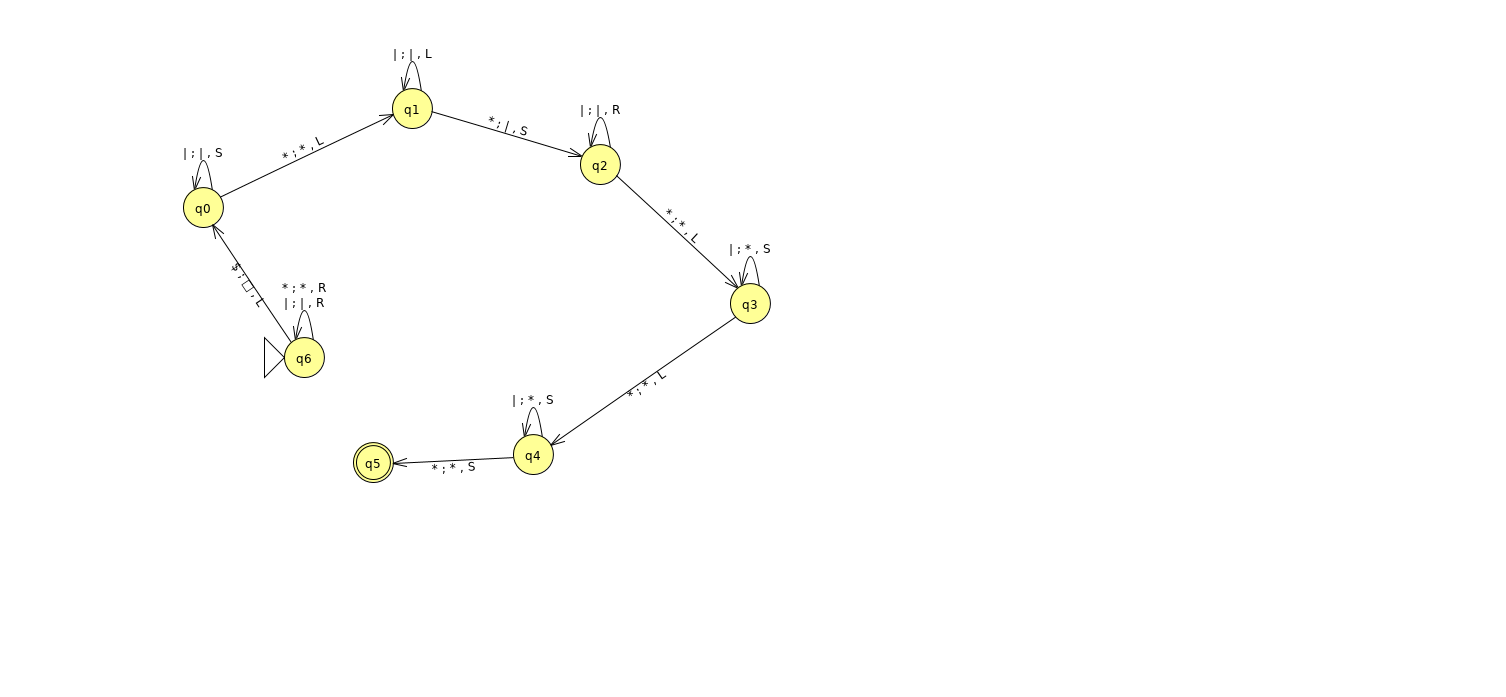
\includegraphics[scale=0.50]{/home/alumno/Descargas/talfuma/ejercicio1_practica3.png}
\caption{}
\end{figure}

\section{Define a recursive function for the sum of three values.}
\begin{center}
addition\_3 = $<<\pi^1_1|\sigma\left(\pi^3_3\right)>|\sigma\left(\pi^4_4\right)>$
\end{center}
\newpage
\begin{figure}[htp]
\centering
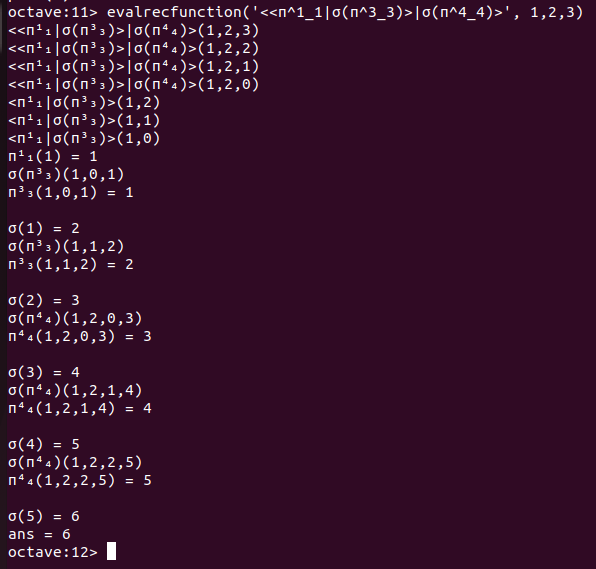
\includegraphics[scale=0.50]{/home/alumno/Descargas/talfuma/ejercicio2_practica3.png}
\caption{}
\label{}
\end{figure}
\section{Implement  a  WHILE  program  that  computes  the  sum  of  three  values.   You
must use an auxiliary variable that accumulates the result of the sum.}

\begin{whilecode}[H]

\ Q=(3,4,s)
\\ s:

 \While{$X_1 \not = 0$}{

  $X_2 \Assig X_2 + 1$\;
  $X_1 \Assig X_1 - 1$

 }
 $X_4 \Assig X_2$
 
  \While{$X_2 \not = 0$}{

  $X_3 \Assig X_3 + 1$\;
  $X_2 \Assig X_2 - 1$

 }
 $X_1 \Assig X_3$
  
 
 
 \end{whilecode}

\end{document}
